
\documentclass[a4paper,11pt]{article}
\usepackage[a4paper, margin=8em]{geometry}

% usa i pacchetti per la scrittura in italiano
\usepackage[french,italian]{babel}
\usepackage[T1]{fontenc}
\usepackage[utf8]{inputenc}
\frenchspacing 

% usa i pacchetti per la formattazione matematica
\usepackage{amsmath, amssymb, amsthm, amsfonts}

% usa altri pacchetti
\usepackage{gensymb}
\usepackage{hyperref}
\usepackage{standalone}

% imposta il titolo
\title{Appunti Fondamenti di Automatica}
\author{Luca Seggiani}
\date{2025}

% disegni
\usepackage{pgfplots}
\pgfplotsset{width=10cm,compat=1.9}

% imposta lo stile
% usa helvetica
\usepackage[scaled]{helvet}
% usa palatino
\usepackage{palatino}
% usa un font monospazio guardabile
\usepackage{lmodern}

% tikz in sans
\tikzset{every picture/.style={/utils/exec={\sffamily}}}

\renewcommand{\rmdefault}{ppl}
\renewcommand{\sfdefault}{phv}
\renewcommand{\ttdefault}{lmtt}

% circuiti
\usepackage{circuitikz}
\usetikzlibrary{babel}

% disponi il titolo
\makeatletter
\renewcommand{\maketitle} {
	\begin{center} 
		\begin{minipage}[t]{.8\textwidth}
			\textsf{\huge\bfseries \@title} 
		\end{minipage}%
		\begin{minipage}[t]{.2\textwidth}
			\raggedleft \vspace{-1.65em}
			\textsf{\small \@author} \vfill
			\textsf{\small \@date}
		\end{minipage}
		\par
	\end{center}

	\thispagestyle{empty}
	\pagestyle{fancy}
}
\makeatother

% disponi teoremi
\usepackage{tcolorbox}
\newtcolorbox[auto counter, number within=section]{theorem}[2][]{%
	colback=blue!10, 
	colframe=blue!40!black, 
	sharp corners=northwest,
	fonttitle=\sffamily\bfseries, 
	title=Teorema~\thetcbcounter: #2, 
	#1
}

% disponi definizioni
\newtcolorbox[auto counter, number within=section]{definition}[2][]{%
	colback=red!10,
	colframe=red!40!black,
	sharp corners=northwest,
	fonttitle=\sffamily\bfseries,
	title=Definizione~\thetcbcounter: #2,
	#1
}

% disponi problemi
\newtcolorbox[auto counter, number within=section]{problem}[2][]{%
	colback=green!10,
	colframe=green!40!black,
	sharp corners=northwest,
	fonttitle=\sffamily\bfseries,
	title=Problema~\thetcbcounter: #2,
	#1
}

% disponi codice
\usepackage{listings}
\usepackage[table]{xcolor}

\lstdefinestyle{codestyle}{
	backgroundcolor=\color{black!5}, 
	commentstyle=\color{codegreen},
	keywordstyle=\bfseries\color{magenta},
	numberstyle=\sffamily\tiny\color{black!60},
	stringstyle=\color{green!50!black},
	basicstyle=\ttfamily\footnotesize,
	breakatwhitespace=false,         
	breaklines=true,                 
	captionpos=b,                    
	keepspaces=true,                 
	numbers=left,                    
	numbersep=5pt,                  
	showspaces=false,                
	showstringspaces=false,
	showtabs=false,                  
	tabsize=2
}

\lstdefinestyle{shellstyle}{
	backgroundcolor=\color{black!5}, 
	basicstyle=\ttfamily\footnotesize\color{black}, 
	commentstyle=\color{black}, 
	keywordstyle=\color{black},
	numberstyle=\color{black!5},
	stringstyle=\color{black}, 
	showspaces=false,
	showstringspaces=false, 
	showtabs=false, 
	tabsize=2, 
	numbers=none, 
	breaklines=true
}

\lstdefinelanguage{javascript}{
	keywords={typeof, new, true, false, catch, function, return, null, catch, switch, var, if, in, while, do, else, case, break},
	keywordstyle=\color{blue}\bfseries,
	ndkeywords={class, export, boolean, throw, implements, import, this},
	ndkeywordstyle=\color{darkgray}\bfseries,
	identifierstyle=\color{black},
	sensitive=false,
	comment=[l]{//},
	morecomment=[s]{/*}{*/},
	commentstyle=\color{purple}\ttfamily,
	stringstyle=\color{red}\ttfamily,
	morestring=[b]',
	morestring=[b]"
}

% disponi sezioni
\usepackage{titlesec}

\titleformat{\section}
{\sffamily\Large\bfseries} 
{\thesection}{1em}{} 
\titleformat{\subsection}
{\sffamily\large\bfseries}   
{\thesubsection}{1em}{} 
\titleformat{\subsubsection}
{\sffamily\normalsize\bfseries} 
{\thesubsubsection}{1em}{}

% disponi alberi
\usepackage{forest}

\forestset{
	rectstyle/.style={
		for tree={rectangle,draw,font=\large\sffamily}
	},
	roundstyle/.style={
		for tree={circle,draw,font=\large}
	}
}

% disponi algoritmi
\usepackage{algorithm}
\usepackage{algorithmic}
\makeatletter
\renewcommand{\ALG@name}{Algoritmo}
\makeatother

% disponi numeri di pagina
\usepackage{fancyhdr}
\fancyhf{} 
\fancyfoot[L]{\sffamily{\thepage}}

\makeatletter
\fancyhead[L]{\raisebox{1ex}[0pt][0pt]{\sffamily{\@title \ \@date}}} 
\fancyhead[R]{\raisebox{1ex}[0pt][0pt]{\sffamily{\@author}}}
\makeatother

\begin{document}

% sezione (data)
\section{Lezione del 15-04-25}

% stili pagina
\thispagestyle{empty}
\pagestyle{fancy}

% testo
\subsubsection{Approssimazione del punto di crossover a 0 dB}
Potrebbe esserci di interesse trovare quando il diagramma del modulo di una risposta in frequenza interseca l'asse a 0 dB.

Preso ad esempio l'esempio della scorsa lezione, che avevamo portato in forma di Bode:
$$
G(s) = 20 \frac{\left( 10s + 1 \right)}{ (s + 1) \left( \frac{s^2}{400} + \frac{s}{20} + 1 \right) } 
$$
possiamo procedere in 2 modi:
\begin{itemize}
	\item Calcolando il valore approssimato ottenuto nell'ultimo zero o polo agente, e l'ultima salita/discesa in dB/oct o dB/dec che osserviamo nel grafico, e quindi cercando l'intersezione del grafico.

		Nell'esempio precedente avremo quindi l'ultimo punto fisso a 46 dB, con una discesa da questo in poi di -40 dB/dec.
		Avremo quindi che l'andamento della risposta in modulo da $\omega = 200$ in poi:
		$$
		|G(j \omega)|_{dB} = 46 - 40 \log\left( \frac{\omega}{20} \right)
		$$
		da cui imponendo a 0:
		$$
		0 = 46 - 40 \log\left( \frac{\omega}{20} \right) \implies \omega^* = 20 \cdot 10^{\frac{46}{40}} \approx 282.51
		$$
		cioè risulta che a $\sim 282.84$ rad/s si ha il punto di intersezione in 0 dB.

	\item Sommando (che in dB significa moltiplicando) le approssimazioni asintotiche di ogni termine al numeratore e denominatore, quindi ogni zero e polo, e imponendo il loro rapporto all'unità (come abbiamo detto, 0 dB significà unità).

		Nell'esempio precedente vorremmo partire dalla costante:
		$$
		G(s) \approx 20
		$$
		e quindi moltiplicare per l'approssimazione asintotica dello zero, che è il solo termine in $s$, $10s$:
		$$
		\approx 20 \cdot 10s = 200s
		$$
		Dividiamo quindi per il polo lineare, prendendo ancora solo il termine in $s$, cioè $s$ stesso:
		$$
		\approx \frac{200s}{s} = 200
		$$
		e infine dividiamo per il polo quadratico, per cui come approssimazione asintotica prendiamo il termine di grado massimo in, $\frac{s^2}{400}$:
		$$
		\approx 200 \cdot \frac{400}{s^2}
		$$
		Imponendo qindi l'unità si ottiene:
		$$
		\frac{80000}{s^2} = 1 \implies s = \sqrt{80000} \approx 282.84
		$$
		cioè risulta a $\sim 282.84$ rad/s si ha il punto di intersezione in 0 dB, che è abbastanza vicino alla stima precedente.
\end{itemize}

\subsection{Luogo delle radici}
Il luogo delle radici è un metodo per studiare sul piano complesso l'effetto della reazione negativa sui poli del sistema in catena chiusa, assunto di conoscere la funzione di trasferimento in catena aperta $G(s)$, cioè secondo quanto già visto in 15.2, da cui riportiamo il grafico:
\begin{center}
	\begin{tikzpicture}
		\draw (1,0) rectangle (3, 1);
		\node at (2, 0.5) {$G(s)$};

		\draw (-3,0) rectangle (-1, 1);
		\node at (-2, 0.5) {$C(s)$};

		\draw (-1.5, -0.5) rectangle (0.5, -1.5);
		\node at (-0.5, -1) {$H(s)$};

		\draw[-stealth] (-7, 0.5) -> (-5.1, 0.5);
		\draw[-stealth] (-5, 0.5) -> (-3, 0.5);
		\draw[-stealth] (-1, 0.5) -> (1, 0.5);
		\draw[-stealth] (3, 0.5) -> (3.9, 0.5);
		\draw[-stealth] (4, 0.5) -> (7, 0.5);

		\draw (5, 0.5) -> (5, -1);
		\draw[-stealth] (5, -1) -> (0.5, -1);
		\draw (-1.5, -1) -> (-5, -1);
		\draw[-stealth] (-5, -1) -> (-5, 0.5);

		\draw[-stealth] (4, 1.5) -> (4, 0.6);
		\node at (4, 1.75) {disturbo};

		\draw[fill=white] (-5, 0.5) circle (0.1);
		\draw[fill=white] (4, 0.5) circle (0.1);

		\node at (-6, 0.75) {$R(s)$};
		\node at (6, 0.75) {$Y(s)$};

		\node at (-4.75, 0.75) {$+$};
		\node at (-4.75, 0.25) {$-$};

		\node at (-3.8, 0.75) {\textit{errore}};
		\node at (0, 0.75) {\textit{controllo}};
		\node at (-3.5, -1.5) {\textit{feedback}};
	\end{tikzpicture}
\end{center}
assunto, come sempre, $H(s)$ sensore all'unità e disturbi trascurabili.

Facciamo quindi l'ulteriore semplificazione di prendere il controllore come una \textit{costante proporzionale}, cioè:
$$
C(s) = K
$$

Il luogo delle radici permette quindi l'analisi \textit{grafico-visuale} delle variazioni dei poli in catena chiusa al variare di uno o più parametri (eventualmente introdotti da un controllore).

\subsubsection{Equazione caratteristica}
Avremo quindi che, sotto le ipotesi di cui sopra, le risposte saranno:
\begin{itemize}
	\item In \textbf{circuito aperto}:
		$$
		K \cdot G(s) = K \cdot \frac{\prod_{i = 1}^m (s - z_i)}{\prod_{i = 1}^n (s - p_i)} = K \cdot \frac{n(s)}{d(s)}
		$$
	\item In \textbf{circuito aperto}:
		$$
		W(s) = \frac{K \cdot G(s)}{1 + K \cdot G(s)} = \frac{K \cdot n(s)}{d(s) + K \cdot n(s)}
		$$
\end{itemize}

I poli in catena chiusa saranno quindi le radici del polinomio:
$$
d(s) + K \cdot n(s)
$$
chiamiamo infatti la seguente equazione:
$$
d(s) + K \cdot n(s) = 0
$$
\textbf{equazione caratteristica} del sistema in catena chiusa.

Il \textbf{luogo delle radici} in sé per sé sarà quindi l'insieme delle radici dell'equazione caratteristica al variare di $K$.

\subsubsection{Regole di tracciamento 1}
Vediamo allora una serie di \textit{regole} che possiamo usare per tracciare il luogo delle radici:

\begin{enumerate}
	\item 
		Varrà quindi la regola (1), cioè che il numero di radici in ciclo chiuso è uguale al numero di poli della funzione $G$ in ciclo aperto.
		Questo significa che il numero di \textit{rami} del luogo delle radici è uguale al numero di poli della funzione di trasferimento in ciclo aperto.

		In particolare, diciamo che il numeratore $n(s)$ ha grado $m$ e il denominatore $d(s)$ ha grado $n$, con $n \geq m$.
		Questo coincide con la definizione che abbiamo dato prima della $G(s)$, che era:
		$$
		G(s) = \frac{\prod_{i = 1}^m (s - z_i)}{\prod_{i = 1}^n (s - p_i)}
		$$
		Avremo allora che l'equazione caratteristica ha grado $n$, cioè si hanno tante radici dell'equazione caratteristica quanti sono i poli della funzione di trasferimento in ciclo aperto.

		\par\medskip
		\noindent
		\textbf{\sffamily{Esempio}}

		Introduciamo la funzione di trasferimento di esempio:
		$$
		G(s) = \frac{1}{s (s + 1)}
		$$
		Cioè:
		$$
		n(s) = 1, \quad d(s) = s(s + 1)
		$$
		in questo caso varrà che $m = 0$ (non ci sono zeri) e $n = 2$, cioè ci aspetteremo di trovare due rami.

	\item	
		La regola (2) riguarda la caratterizzazione geometrica del luogo delle radici. Riprendendo l'equazione caratteristica, potremo infatti dire:
		$$
		d(s) + K \cdot n(s) = 0 \implies \frac{n(s)}{d(s)} = -\frac{1}{K}
		$$
		Da questa ricaviamo due condizioni di appartenenza al luogo delle radici, rispettivamente in \textit{fase} e in \textit{modulo}.
		\begin{itemize}
			\item 
				Si definisce la cosiddetta \textbf{condizione di fase}:
				\[
					\begin{cases}
						\angle n(s) - \angle d(s) = -\pi \pm 2 h \pi, \quad K > 0 \\
						\angle n(s) - \angle d(s) = \pm 2 h \pi, \quad K < 0
					\end{cases}
				\]
				Questa deriva dal fatto che. per le proprietà stesse del prodotto complesso, vale:
				$$
				\angle \left( \frac{n(s)}{d(s)} \right) = \angle n(s) - \angle d(s)
				$$
				mentre il termine a destra, essendo $K$ un reale, sarà $-\pi$ se $K > 0$, e $0$ viceversa.
				I termini $2 h \pi$, con $h \in \mathbb{N}$, vengono introdotti perché ruotando di $360^\circ$ gradi sul piano complesso si torna da dove si è partiti.
				Vediamo quindi che applicare la condizione di fase significa costruire il luogo delle radici, cioè questa condizione da sola basta a ricavare tutto il luogo.

				Possiamo dare un'ulteriore interpretazione geometrica degli angoli.
				Si ha infatti che vale, sempre per le proprietà dei complessi, rispetto a un qualsiasi punto $s$:
				\[
					\begin{cases}
						\angle n(s) = \arg \prod_{i = 1}^m (s + z_i) = \sum_{i = 1}^m (s + z_i) = \sum_{i = 1}^m \theta_i \\ 
						\angle d(s) = \arg \prod_{j = 1}^n (s + p_j) = \sum_{j = 1}^n (s + p_j) = \sum_{j = 1}^n \phi_j 
					\end{cases}
				\]
				dove $\phi_j$ e $\theta_i$ rappresentano gli angoli le congiungenti con i poli in $j$ e gli zeri in $i$ formano con l'asse reale. 

				\par\medskip
				\noindent
				\textbf{\sffamily{Esempio}}

				Riprendiamo il polinomio:
				$$
				G(s) = \frac{1}{s (s + 1)}
				$$
				possiamo anticipare che i suoi poli sono $p_1 = 0$ e $p_2 = -1$.
				In questo caso, preso ad esempio il punto $s = -\frac{1}{2} + i$ si avranno gli angoli:

				\begin{center}
					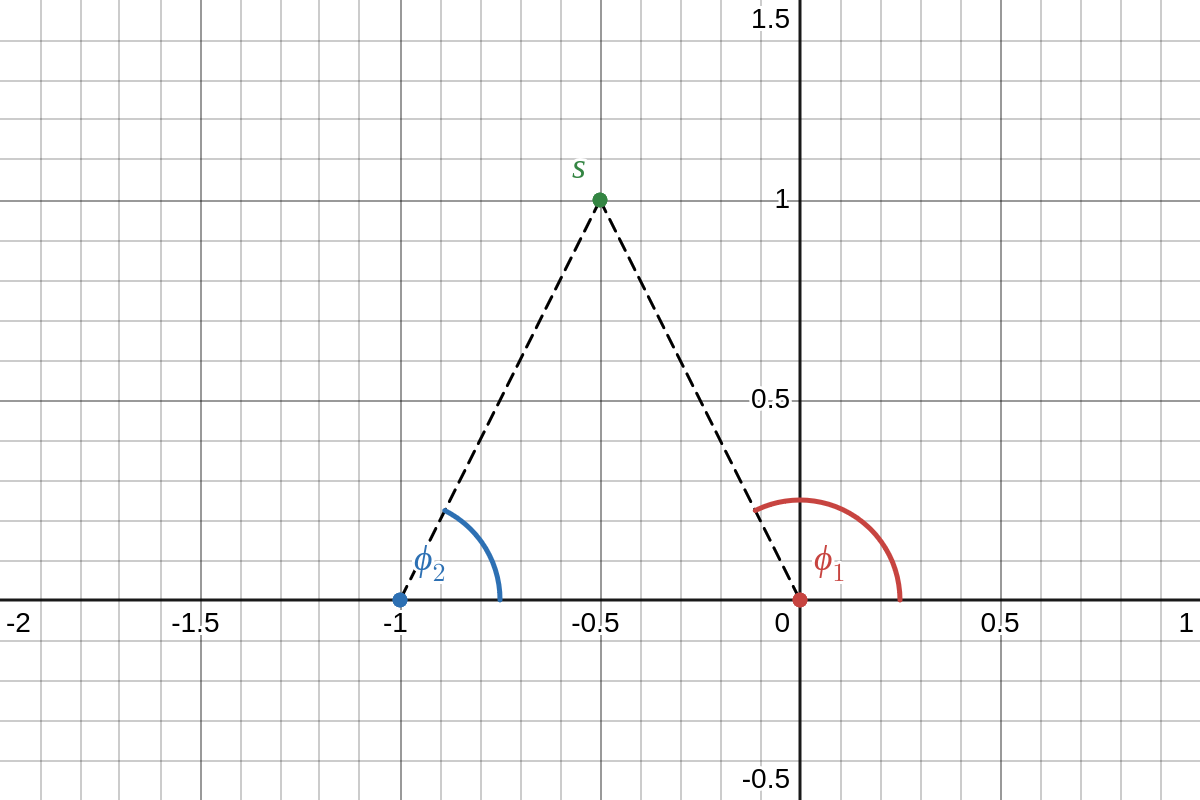
\includegraphics[scale=0.26]{../figures/locus_phi.png}
				\end{center}

			\item
				Nessuno ci nega di costruire anche una \textbf{condizione di modulo}, cioè imporre ai soli moduli:
				$$
				\left| \frac{n(s)}{d(s)} \right| = \frac{1}{|K|}
				$$
				Vediamo che questa condizione non è indispensabile, ma invece applicarla significa "tarare" il luogo delle radici su un singolo valore di $K$.

				Abbiamo anche qui un'interpretazione geometrica analoga a quella degli angoli.
				Potremo infatti dire:
				$$
				|n(s)| = \prod_{i = 1}^m |s + z_i|, \quad |d(s)| = \prod_{i = 1}^n |s + p_i|
				$$
				dove gli $|s^* + z_i| = \lambda_i$ e $|s^* + p_i| = \eta_i$ corrispondono alle distanze del generico punto nel luogo $s^*$, per cui:
				$$
				|K| = \frac{ \prod_{i = 1}^n |s^* + p_i| }{ \prod_{i = 1}^m |s^* + z_i| } = \frac{ \prod_{i = 1}^n \eta_i }{ \prod_{i = 1}^m \lambda_i }
				$$
				Cioè il guadagno $K$ per un certo punto $s^*$ corrisponde al rapporto fra il prodotto delle distanze dai poli e il prodotto delle distanze dagli zeri.

				\par\medskip
				\noindent
				\textbf{\sffamily{Esempio}}

				Riprendiamo il polinomio:
				$$
				G(s) = \frac{1}{s (s + 1)}
				$$
				conosciamo i suoi $p_1 = 0$ e $p_2 = -1$.
				In questo caso, preso lo steso punto $s = -\frac{1}{2} + i$ di prima (che anticipiamo far parte del luogo) si avranno le distanze:

				\begin{center}
					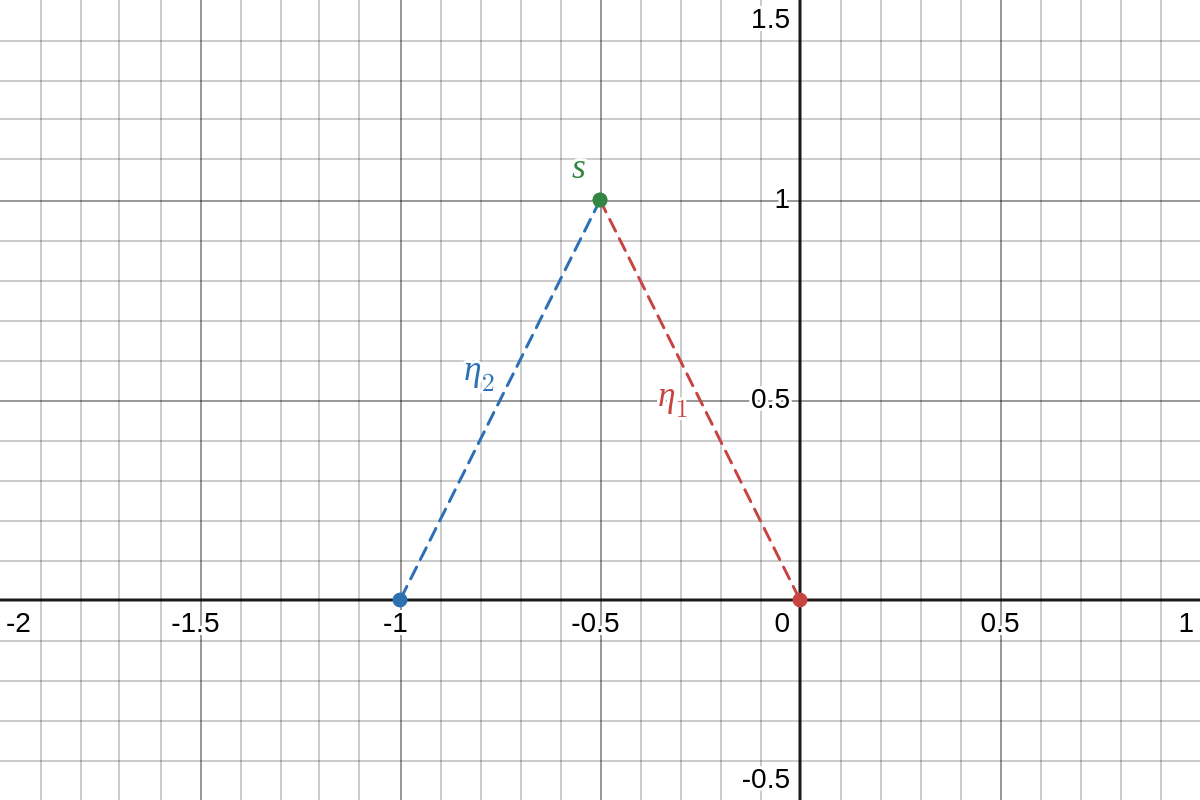
\includegraphics[scale=0.26]{../figures/locus_eta.png}
				\end{center}

		\end{itemize}

	\item
		Potremo quindi ricavare la regola (3), che riguarda l'andamento in funzione di $K$ del luogo, cioè dire che preso:
		$$
		d(s) + K \cdot n(s) = 0
		$$
		ponendo $K = 0$ si nota che il luogo parte dai \textbf{poli a ciclo aperto} del sistema (cioè da $d(s) = 0$);

		Di contro, preso:
		$$
		\frac{1}{K} \cdot d(s) + n(s) = 0
		$$
		ponendo $K = +\infty$ si nota che il luogo arriva agli \textbf{zeri a ciclo aperto} del sistema (cioè $n(s) = 0$).

		Si ha quindi la regola generale che il luogo \textit{parte} dai \textbf{poli a ciclo aperto} e \textit{arriva} agli \textbf{zeri a ciclo aperto}.
		
		Questi ultimi, in particolare, possono essere al \textit{finito} o all'\textit{infinito}.
		In particolare, si ha che in presenza di $m$ zeri, $m$ dei rami trovati (ricordiamo $m \leq n$) vanno a finire negli zeri del ciclo aperto, e gli altri $n - m$ divergono ad infinito.

		\par\medskip
		\noindent
		\textbf{\sffamily{Esempio}}

		Riprendiamo l'esempio:
		$$
		G(s) = \frac{1}{s (s + 1)}
		$$
		da cui :
		$$
		K \cdot G(s) = \frac{K}{s (s + 1)} 
		$$
		e quindi l'equazione caratteristica:
		$$
		s(s + 1) + K = 0
		$$
		Posto $K=0$ si trovano quindi i poli in ciclo aperto, cioè punti di partenza del luogo delle radici, $p_1 = 0$ e $p_2 = -1$.
		Per quanto riguarda gli zeri, invece, abbiamo che questi non esistono, quindi dovrmo affidarci ad altre regole per capire l'estensione dei rami.

	\item
		La regola (4) è che tutto l'asse reale appartiene al luogo delle radici, fatta la distinzione fra \textit{Luogo Diretto} (LD) e \textit{Luogo Inverso} (LI):
		\begin{itemize}
			\item \textbf{Luogo Diretto} (LD): ne fanno parte i punti che rispettano la condizione di fase per $K > 0$; 
			\item \textbf{Luogo Inverso} (LI): ne fanno parte i punti che rispettano la condizione di fase per $K < 0$; 
		\end{itemize}
		Notiamo che riguardo alla regola (1), gli $n$ rami sono tali sia per il luogo diretto che per il luogo inverso, cioè l'unione del luogo diretto del luogo inverso conta $2n$ rami complessivi.

		Si ha quindi che l'unione fra luogo diretto e luogo inverso di una certa funzione di trasferimento copre tutto l'asse reale.

		In particolare, se $K > 0$, il luogo lascia alla propria destra un numero \textit{dispari} di punti critici (poli e zeri) sull'asse reale, mentre se $K < 0$, il luogo ne lascia alla propria destra un numero \textit{pari}.

		Questa regola deriva direttamente dalla condizione di fase, che avevamo imposto come:
		\[
			\begin{cases}
				\angle n(s) - \angle d(s) = -\pi \pm 2 h \pi, \quad K > 0 \\
				\angle n(s) - \angle d(s) = \pm 2 h \pi, \quad K < 0
			\end{cases}
		\]

		Si ha quindi che un punto $s$ nel piano di Gauss appartiene al luogo delle radici se la somma delle fasi dei vettori che partono dalle singolarità (poli o zeri) e terminano nel punto $s$ è uguale a $-\pi$ (o 0, se $K < 0$).

		\par\medskip
		\noindent
		\textbf{\sffamily{Esempio}}

		Nel nostro esempio consideravamo: 
		$$
		\angle \frac{1}{s(s + 1)} = \angle 1 - \angle s(s + 1) = -\angle s (s + 1)
		$$
		\begin{itemize}
			\item Per $K > 0$ (luogo diretto) imponiamo quindi la condizione:
				$$
				-\angle s (s + 1) = -\pi \pm 2 h \pi
				$$
				che è rispettata per tutti gli $s \in \mathbb{R}$ con $p_2  \leq s \leq p_1$.

				\newpage

				In questo caso si ha quindi la parte dell'asse reale:
				\begin{center}
					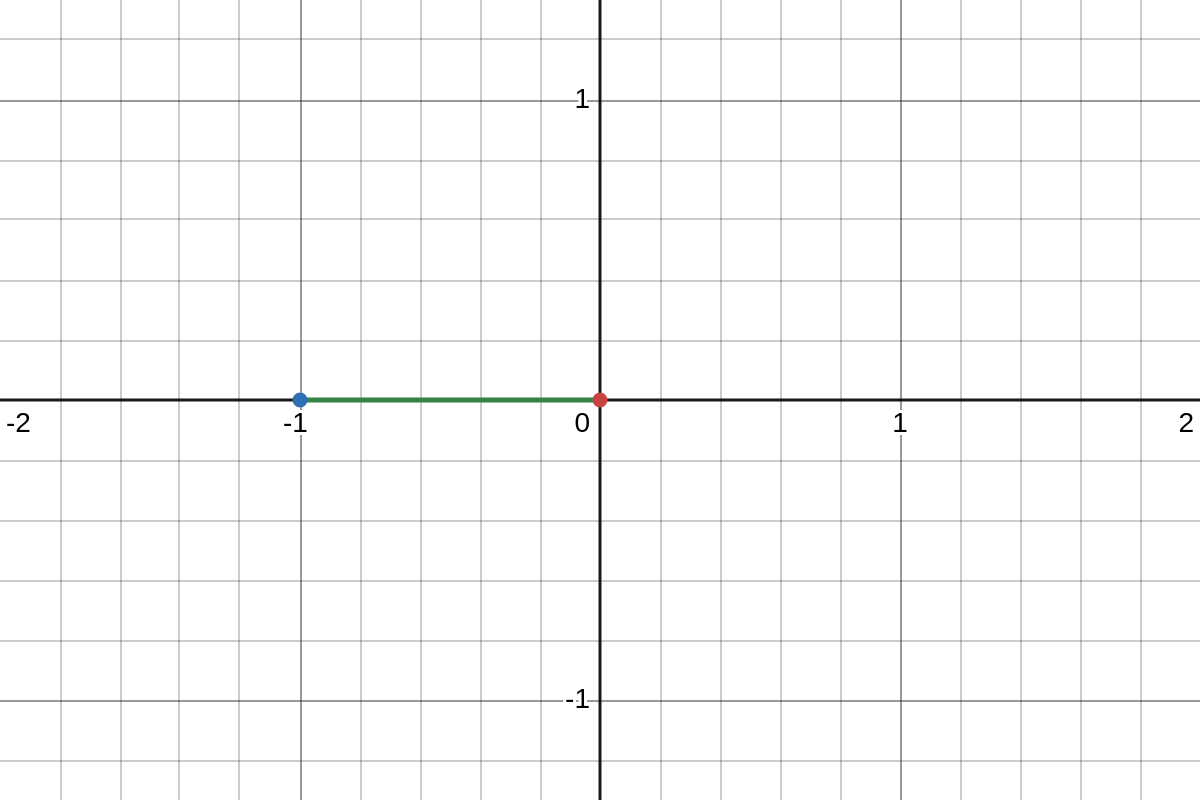
\includegraphics[scale=0.26]{../figures/locus_dr.png}
				\end{center}

				Abbiamo quindi preso tutti gli $s$ che hanno un numero \textbf{dispari} di poli a destra.

			\item Per $K < 0$ (luogo inverso) imponiamo invece la condizione:
				$$
				-\angle s (s + 1) =\pm 2 h \pi
				$$
				che è rispettata per tutti gli $s \in \mathbb{R}$ con $s \leq p_2$ o $s \geq p_1$.

				In questo caso si ha quindi la parte dell'asse reale:
				\begin{center}
					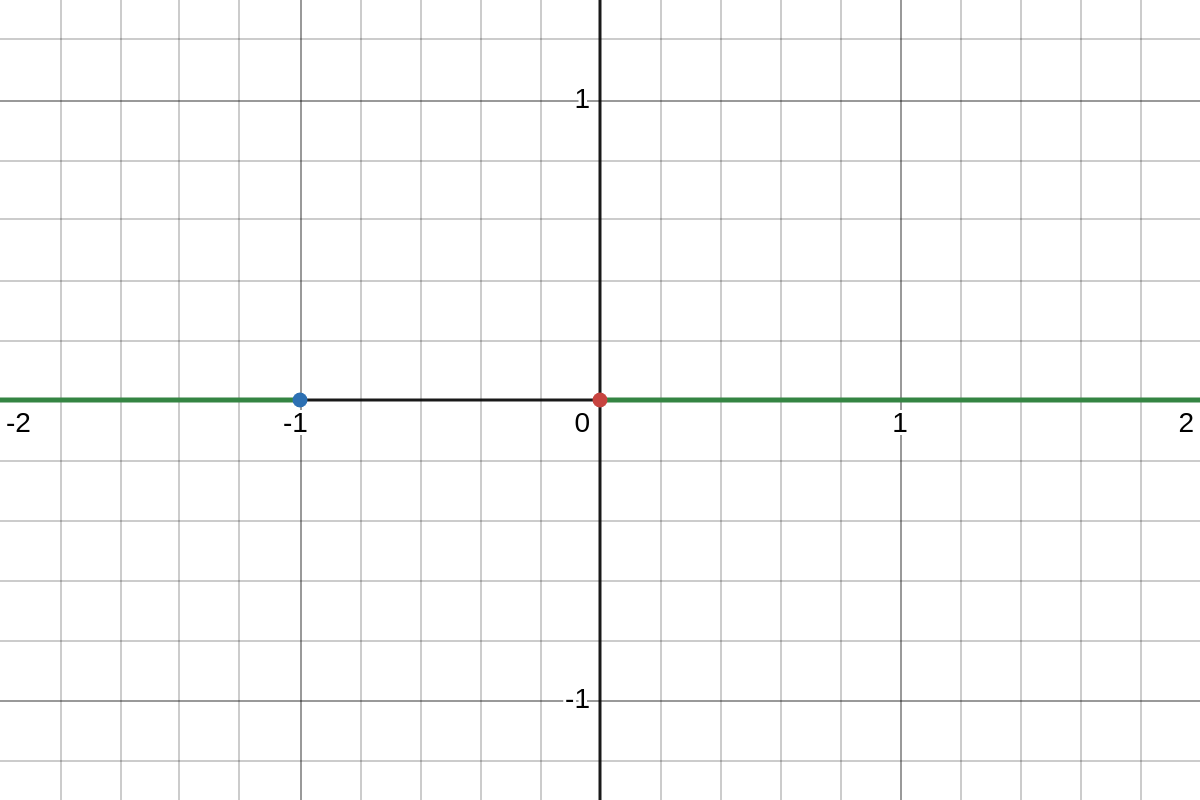
\includegraphics[scale=0.26]{../figures/locus_ir.png}
				\end{center}

				Abbiamo quindi preso tutti gli $s$ che hanno un numero \textbf{pari} di poli a destra.
		\end{itemize}

	\item
		La regola (4) afferma che il luogo delle radici è \textbf{simmetrico} rispetto all'\textit{asse reale}.
		Questo deriva direttamnente dal fatto che l'equazione caratteristica è reale, quindi ammetterà soluzioni reali o complesse coniugate.

		Vediamo quindi che dalla regola (2) rispetto agli angoli, tutto l'asse del segmento del luogo diretto sarà parte del luogo, in quanto avremo due angoli $\phi_1$ e $\phi_2$ ai poli fra di loro complementari (è questo proprio il caso che abbiamo preso ad esempio della regola (2)).
		In particolare potremmo dire, dati $\phi_1$ e $\phi_2$ complementari:
		$$
		-(\phi_1 + \phi_2) -(\phi_1 + (\pi - \phi_1)) = -\pi \pm 2 h \pi
		$$
		che chiaramente è rispettato per $h = 0$ (i meno vengono dal fatto che prendiamo poli al denominatore).

		Potremo quindi estendere il luogo diretto a (dove nel grafico si sono disegnati anche gli angoli complementari):
		\begin{center}
			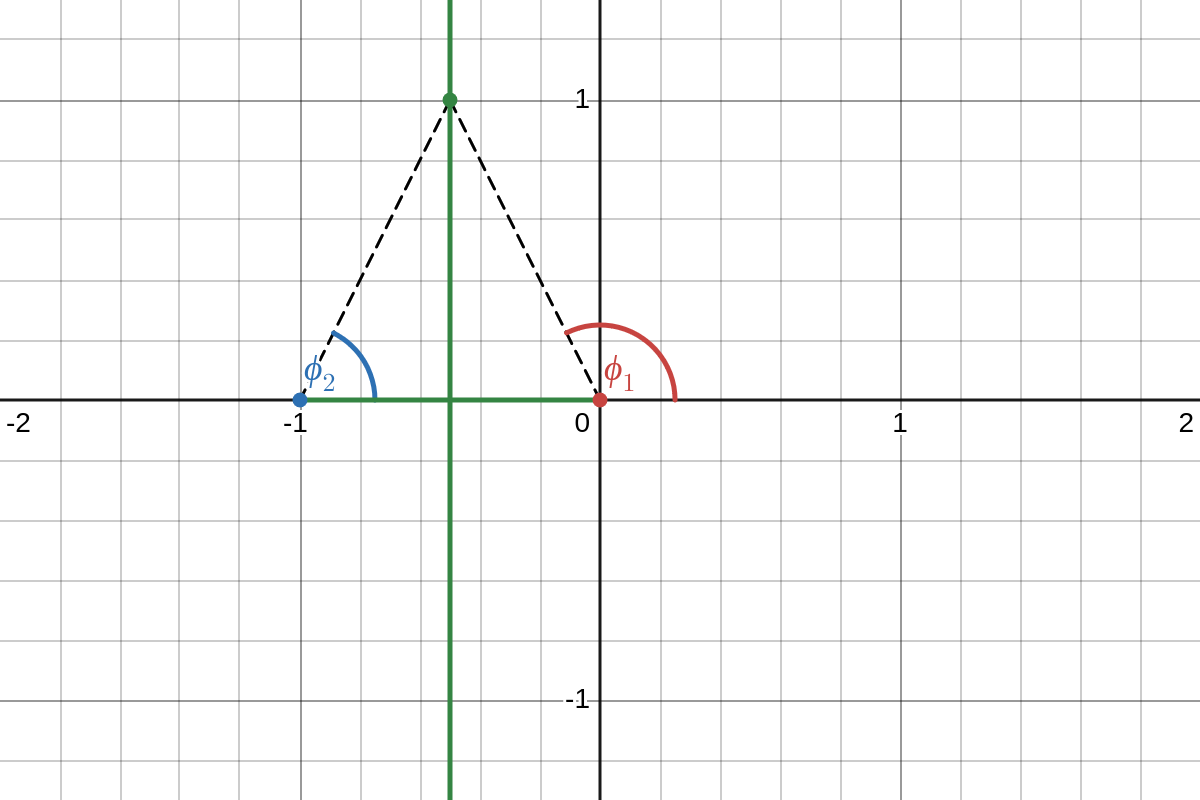
\includegraphics[scale=0.26]{../figures/locus_dc.png}
		\end{center}
		
		Notiamo che in ogni caso i rami sia del luogo diretto che del luogo inverso sono 2, come dalla regola (1).
\end{enumerate}

\end{document}
